\chapter{Umsetzung}

\section{Aktueller Stand der LSY}
\begin{figure}[h]
	\centering 
	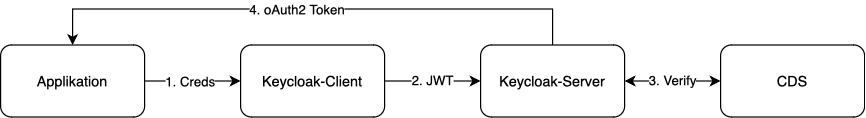
\includegraphics[width=1\textwidth]{img/abbildungen/Unknown.png}
	\captionsetup{format=hang}
	\caption{Aktuelle Umsetzung der Abteilung}
\end{figure}

\begin{itemize}
    \item Innerhalb der Abteilung wird eine passwortbasierte Authentifizierung durchgeführt, welche zusätzlich durch \ac{MFA} geschützt wird.
    \item Webanwendung nutzt einen eigene Anwendung, welche sich als Keycloak-Client aussgibt. Der Nutzer gibt seine Zugangsdaten an den Keycloak-Client weiter, welche diese verarbeitet. Dieser wandelt die Zugangsdaten in einen validen JWT-Token um und übergibt diesen an den Keycloak-Server. Dieser validiert die Zugangsdaten gegen die \ac{CDS}. Ist die Validierung erfolgreich, wird vom Keycloak-Server ein oAuth2-Token erstellt und zurück an die Applikation übergeben.
    \item Innerhalb der \ac{LSY} können sich Applikationen allerdings auch gegen das Azure \ac{AD} authentifizieren lassen. 
\end{itemize}

\section{Wahl des Security Keys}
Für die Umsetzung der passwortlosen Authentifizierung innerhalb der \ac{LSY} wurde ein Yubikey der Series 5 mit NFC gewählt. Dieser wurde in Kapitel vorgestellt. Hingewiesen sei an dieser Stelle darauf, dass auch andere Hersteller Security Keys anbieten, welche das Fido2-Protokoll unterstützen. 

Weitere bekannte Security Keys sind unter anderem:
\begin{itemize}
    \item \textit{Feitian ePass} des Herstellers FEITIAN Technologies Co., Ltd.
    \item \textit{Titan} des Herstellers Google
    \item \textit{SafeNet eToken} des Herstellers Thales Group
\end{itemize}

Die Wahl des Security Keys richtete sich allerdings unter anderem an der Kompatibilitätsliste \cite{compWin} von Microsoft. Diese listet alle Security Keys auf, welche für eine passwortlose Authentifizierung gegen eine Microsoft Azure \ac{AD} genutzt werden können. Nicht auffindbar in der Liste ist beispielsweise der Google Titan. Dieser unterstützt aktuell nicht FIDO2, sondern lediglich FIDO und \ac{U2F}. Microsoft ist allerdings nich abwärtskompatibel, was bedeutet, dass der Google Titan nicht für eine passwortlose Authentifizierung gegen das Azure \ac{AD} genutzt werden kann \cite{seckeytest}.

Die endgültige Auswahl basiert  auf dem bestehenden Bestand eines Yubikeys der Series 5 mit NFC. Dieser ist mit der Azure \ac{AD} nutzbar. Grundsätzlich ist allerdings auch eine Nutzung eines anderen Security Keys möglich, sofern dieser das \ac{FIDO}2-Protokoll unterstützt, in der Kompatibilitätsliste von Microsoft aufgeführt ist und und offiziel von der \ac{FIDO} Allianz zertifiziert wurde.

\section{Integration eines Yubikeys in die LSY}

\begin{figure}[h]
	\centering 
	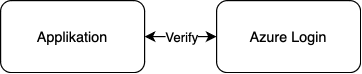
\includegraphics[width=0.6\textwidth]{img/abbildungen/azure_umsetzung.png}
	\captionsetup{format=hang}
	\caption{Umsetzungsmöglichkeit mit Azure \ac{AD}}
\end{figure}

\begin{itemize}
    \item Grundsätzlich gibt es zwei Möglichkeiten in die aktuelle Applikation eine passwortlose Authentifizierung mit Hilfe eines Yubikeys zu integrieren: Die Nutzung der Authentifizierung gegen das Azure \ac{AD} oder die eine veränderte Nutzung der aktuellen Keycloak-Lösung.

\end{itemize}

Eine Lufthansa-weite Policy für die Nutzung der Azure \ac{AD} verbietet allerdings die Nutzung eines Security Keys für eine \ac{SFA}. Hier kann der Security Key lediglich als zweiter Faktor genutzt werden. Dies kann jeder Nutzer selber verwalten. Registriert ein Nutzer seinen Security Key in seinem Profil, erscheint bei der Anmeldung (nach der Eingabe des Passwortes) ein zusätzliches Feld:

\begin{figure}[h]
	\centering 
	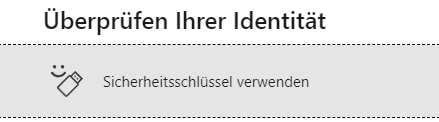
\includegraphics[width=0.6\textwidth]{img/abbildungen/azure_seckey.png}
	\captionsetup{format=hang}
	\caption{Umsetzungsmöglichkeit mit Keycloak}
\end{figure}

Verwendet der Nutzer einen Security Key wird dieser im Folenden aufgefordert die zugehörige PIN einzugeben und den Knopf des Security Keys zu drücken. Grundsätzlich ist eine passwortlose Authentifizierung mit Hilfe eines Security Keys innerhalb der Azure \ac{AD} möglich. Da eine Änderung dieser Lufthansa Policy notwendig wäre, übersteigt dies allerdings den Rahmen dieser Arbeit.

Da allerdings aktuell eine beschriebene Nutzung von Keycloak stattfindet und Keycloak eine passwortlose Authentifizierung mit Hilfe eines Security Keys unterstützt, wäre eine Umsetzung mit Hilfe von Keycloak möglich. Hierbei wird die aktuelle Lösung verändert und entsprechend angepasst:

\begin{figure}[h]
	\centering 
	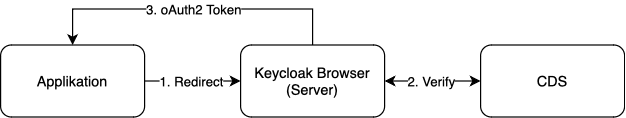
\includegraphics[width=1\textwidth]{img/abbildungen/keycloak_browser.png}
	\captionsetup{format=hang}
	\caption{Veränderter Keycloak-Login}
\end{figure}

Statt bei einer Anmeldung einen Client zu simulieren bietet Keycloak die Möglichkeit eine Anmeldung über eine Nutzeroberfläche zu realisieren. Dafür wird ein redirect auf die Keycloak-Login-Seite durchgeführt. Bei einer erfolgreichen Verifizierung wird der Nutzer zurück auf die Applikation geleitet und vom Keycloak-Server mit Hilfe eines oAuth2-Tokens authentifiziert. 

Um eine Passwortlose Authentifizierung in Keycloak zu ermöglichen, muss der Authentication Flow für eine Browser-Anmeldung modifiziert werden. Der angepasste Authentication Flow besteht aus folgenden Schritten:

\begin{figure}[h]
	\centering 
	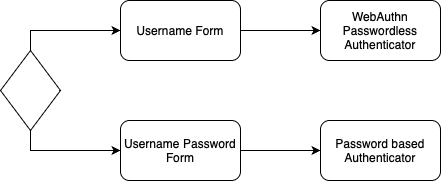
\includegraphics[width=0.7\textwidth]{img/abbildungen/authentication_flow.png}
	\captionsetup{format=hang}
	\caption{Authentication Flow}
\end{figure}

Hierbei wird die untere Hälfte der Grafik weiterhin ermöglicht, da es sich lediglich um einen Test handelt. Grundsätzlich wird diese nicht ermöglicht, da Keycloak eine reine passwortlose \ac{SFA} unterstützt.

Die obere Hälfte der Grafik entspricht dem für diese Arbeit relevanten Authentication Flow. Dabei wird der User zunächst aufgefordert seinen Nutzernamen einzugeben und anschließend seinen Security Key zu verwenden. Dies ist notwendig, um die Nutzung eines Security Keys für mehrere Zugänge zu ermöglichen. Ermöglicht man lediglich die Nutzung eines Zugangs pro Security Key, so wird die Eingabe des Nutzernamens nicht benötigt. Zusätzlich erfolgt eine Konfiguration des Keycloak-Servers, welche die Registrierung eines Security Keys bei der Registrierung eines neuen Nutzers ermöglicht.

Mit Hilfe dieser Konfiguration werden zwei Abläufe ermöglicht. Eine neue Registrierung:

\begin{figure}[H]
	\centering 
	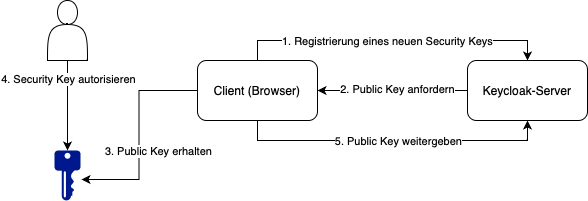
\includegraphics[width=1\textwidth]{img/abbildungen/register_simplified.png}
	\captionsetup{format=hang}
	\caption{Registrierung (vereinfacht)}
\end{figure}

Sowie eine neue Anmeldung:

\begin{figure}[H]
	\centering 
	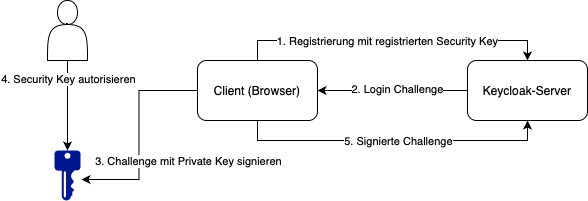
\includegraphics[width=1\textwidth]{img/abbildungen/login_simplified.png}
	\captionsetup{format=hang}
	\caption{Anmeldung (vereinfacht)}
\end{figure}

Die Grafiken stellen den vereinfachten Ablauf der Registrierung und Anmeldung mit Hilfe eines Security Keys dar. Die detailierte Darstellung der Funktionsweise ist in Kapitel 2.7 zu finden. Der entscheidende Unterschied der beiden Prozesse ist allerdings, dass bei der Registrierung lediglich der öffentliche Schlüssel übergeben wird, während bei der Anmeldung der private Schlüssel benötigt wird. Dieser wird allerdings nicht übergeben, sondern signiert eine Login Challenge, welche vom Keycloak-Server generiert wird. Kann der Keycloak-Server die Signatur mit Hilfe des gespeicherten öffentlichen Schlüssels verifizieren, wird der Nutzer authentifiziert. Sowohl die Registrierung als auch die Anmeldung erfolgen hierbei also nicht über die Anwendung selbst, sondern über den Keycloak-Server und dessen Nutzeroberfläche.

\section{User Feedback}
Um eine Aussage über die Akzeptanz und die Benutzerfreundlichkeit der aufgezeigten Umsetzung zu treffen, wird ein Feedback von den Nutzern der Abteilung cGroup Solutions eingeholt. Um eine wissenschaftliche Aussage zu treffen wird ein Fragebogen erstellt. Es handelt sich dabei um eine Mischform aus einer qualitativen und einer quantitativen Befragung. So wird es ermöglicht eine numerische Auswertung der Antworten zu erhalten, sowie eine qualitative Auswertung der Kommentare. Im Folgenden wird die Durchführung des Fragebogens beschrieben.

\subsection{Rahmen des Feedbacks}
Da zum Zeitpunkt der Erstellung dieser Arbeit die Nutzung keine Umsetzung einer passwortlosen Authentifizierung innerhalb der gesamten \ac{LSY} möglich ist (siehe Kapitel) wird das Feedback auf die Abteilung cGroup Solutions beschränkt. Diese ist zuständig für das in Kapitel beschriebene Produkt cFront, in welchem die passwortlose Authentifizierung testweise implementiert wurde. Die Abteilung besteht aus 15 Personen.

Über einem Zeitraum von zwei Wochen werden alle Mitglieder eingeladen an der Befragung teilzunehmen. Eine Teilnahme ist freiwillig. Die Befragung findet im Büro der Abteilung statt und wird von dem Autor dieser Arbeit durchgeführt. Jeder Teilnehmer wird einzeln und vor Ort befragt. Dies ermöglicht es mit jedem Teilnehmer eine Live-Demonstration durchzuführen. So wird ebenfalls ermöglicht, dass Teilnehmer bereits während der Befragung und der Demonstration Kommentare hinterlassen können. Diese werden auf dem Fragebogen festgehalten und werden für die qualitative Auswertung genutzt werden.

Während der gesamten Demonstration und Befragung werden den Teilnehmern keine Informationen zum Fido2 Protkoll vermittelt, da sonst die Aussagekraft des Feedbacks verfälscht werden könnte. Ziel ist es den ersten Eindruck aller Teilnehmer zu erhalten, ohne dass diese eine erzwungene Einführung in die Thematik erhalten. Die Live-Demonstration beinhaltet die Registrierung und Anmeldung mit Hilfe eines Security Keys, sowie eine Demonstration einer möglichen Anmeldung mit Hilfe eines Passkeys. Zusätzlich erhalten die Teilnehmer die Möglichkeit den Security Key physich zu betrachten. Ein detailierter Verlauf der Demonstartion wird im weiteren Verlauf der Arbeit beschrieben.

\subsection{Auswahl der Teilnehmer}
Zur Durchführung des Fragebogens wurden alle Mitglieder des Teams eingeladen, eine Teilnahme war jedoch freiwillig. Zwei der Mitglieder der Abteilung konnten auf Grund eines Urlaubs nicht an der Befragung teilnehmen. Vor der Durchführung wurden alle Teilnehmer darüber informiert zu welchem Zweck die Daten für diese Arbeit erhoben werden. Die Befragung stand dabei nicht anonym statt, um einen Austausch zwischen dem Autor und den Teilnehmern zu ermöglichen. Da die Befragung die Abteilung der Teilnehmer betrifft sollten diese somit eine Möglichkeit bekommen, ihre Gedanken zu dem modifiziertem Anmeldevorgang zu teilen.

14 Mitglieder der Abteilung stimmten der Teilnahme an der Befragung zu. Die letzte Person befand sich während des möglichen Zeitraumes der Befragung im Urlaub. Das durchschnittsalter der Teilnehmer beträgt xy Jahre. Die genaue Verteilung wird in der folgenden Grafik sichtbar:

Dabei ist auffällig, dass die Teilnehmer der Befragung überwiegend der Gruppe 50-60 Jahre zugehörig sind. Auch die Gruppe 20-30 Jahre ist häufig vertreten. Lediglich die Gruppe 40-50 Jahre ist wenig vertreten. Daraus lässt sich schließen, dass die Teilnehmer der Befragung überwiegend entweder neu in das Berufsfeld eingestiegen sind oder bereits eine langjährige Erfahrung in diesem Bereich haben. 

Vor Beginn der Befragung wurden die Teilnehmer gebeten anzugeben, welche Rolle sie innerhalb des Teams einnehmen. Daraus lassen sich zwei Gruppen bilden: Development und Operations. Die Verteilung der Teilnehmer auf die beiden Gruppen ist in der folgenden Grafik dargestellt:

\subsection{Inhalt der Demonstration}
Allen Teilnehmern wurde vor der Befragung eine Live-Demonstration der Registrierung und Anmeldung mit Hilfe eines Security Keys gezeigt. Der Security Key wurde zu Beginn der Demonstration in einen üblichen USB-Slot eines Firmenlaptops eingesteckt und nach der Demonstration an die Teilnehmer übergeben. 

Die Anmeldung/Registrierung ist in mehrere Schritte unterteilt. Zunächst bestätigt der Nutzer, dass er sich mit Hilfe eines Security Keys anmelden/registrieren möchte:

\begin{figure}[h]
	\centering 
	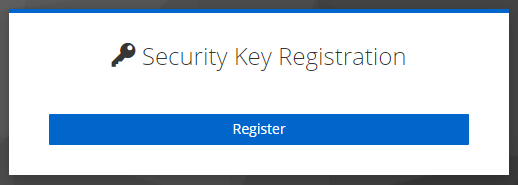
\includegraphics[width=0.7\textwidth]{img/abbildungen/reg001.png}
	\captionsetup{format=hang}
	\caption{Veränderter Keycloak-Login}
\end{figure}

Darauf folgt ein Dialogfeld des Browsers, welcher den Nutzer dazu auffordert zu bestätigen, dass der Security Key registriert wird. Dieser Schritt ist einmalig und findet nur bei der Registrierung statt. Ist der Security Key bereits registriert, wird dieser Schritt übersprungen:

\begin{figure}[h]
	\centering 
	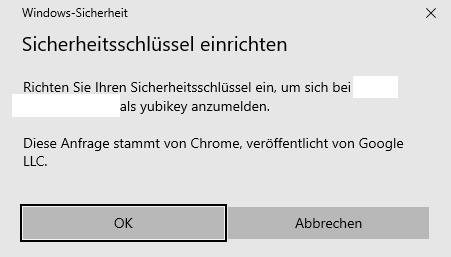
\includegraphics[width=0.7\textwidth]{img/abbildungen/reg002.png}
	\captionsetup{format=hang}
	\caption{Veränderter Keycloak-Login}
\end{figure}

Nach der Bestätigung des Dialogs muss der Nutzer den PIN des Security Keys eingeben:

\begin{figure}[H]
	\centering 
	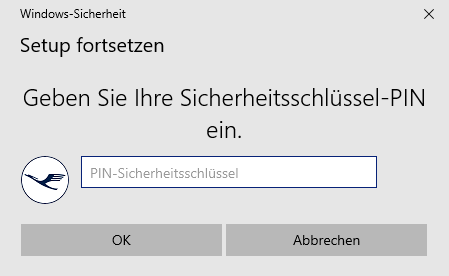
\includegraphics[width=0.7\textwidth]{img/abbildungen/reg003.png}
	\captionsetup{format=hang}
	\caption{Veränderter Keycloak-Login}
\end{figure}

Ist die richtige PIN eingegeben wurden, erscheint ein letztes Fenster, welches den Nutzer dazu auffordert den Knopf des Security Keys zu drücken. Erst danach ist der Browser dazu autorisert sich mit Hilfe des Security Keys gegen den Keycloak-Server zu registrieren oder anzumelden:

\begin{figure}[h]
	\centering 
	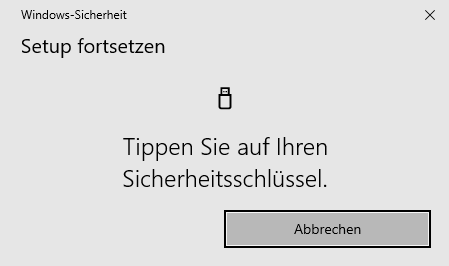
\includegraphics[width=0.7\textwidth]{img/abbildungen/reg004.png}
	\captionsetup{format=hang}
	\caption{Veränderter Keycloak-Login}
\end{figure}

Sobald der Knopfdruck erfolgt, wird der Nutzer erfolgreich eingeloggt. Diese Informationen wurden den Teilnehmern ebenfalls während der Durchführung des Fragebogens mitgeteilt. 


\subsection{Herleitung der Fragen}
Aufgrund des Ziels der Befragung, eine Aussage über die Akzeptanz und die Benutzerfreundlichkeit einer passwortlosen Authentifizierung zu treffen, werden lediglich Fragen gestellt, die sich auf diese beiden Punkte beziehen. Um eine hohe Teilnahme zu gewährleisten, werden die Fragen möglichst kurz gehalten und nur wenige Fragen gestellt. Die Fragen werden so gestaltet, dass sie dem Teilnehmer die Möglichkeit bietet Kommentare zu hinterlassen oder seine Antwort zu begründen. Die Fragen werden so gestellt, dass sie einfach zu verstehen sind und kein Vorkenntnisse im Bereich der passwortlosen Authentifizierung voraussetzen. Im folgenden werden die Fragen begründet aufgelistet und erläutert:

\paragraph{Frage 1:}

\begin{quote}
    \textit{Hast du schonmal einen Security Key genutzt?}
\end{quote}
\textbf{Antwörtmöglichkeiten:} Ja; Nein; 

Diese Frage leitet sich aus \cite{farke2020you} ab. Die Antwortmöglichkeiten werden im Vergleich aber angepasst und reduziert. Durch die Reduzierung auf zwei Antwortmöglichkeiten wird eine bessere Auswertung ermöglicht. Antworten Teilnehmer mit \textit{Ja}, werden sie gefragt in welchem Kontext sie den Security Key genutzt haben. So lassen sich zusätzliche Informationen über die Nutzungsdauer und den Zweck der Nutzung zu erhalten.

\paragraph{Frage 2:}

\begin{quote}
    \textit{Bist du generell bereit deine Passwörter durch eine andere Art der Authentifizierung zu ersetzen?}
\end{quote}
\textbf{Antwörtmöglichkeiten:} Ja; Nein; 

Diese Frage ergibt sich aus einer Umfrage von Statista, in welcher Teilnehmer gefragt wurden, durch welche Art der Authentifizierung sie das Passwort ersetzen würden. Lediglich 22\% der Teilnehmer gaben an, dass sie ihr Passwort lieber beibehalten würden \cite{techstat}. Daraus folgt die Annahme, dass eine Vielzahl an Nutzern grundsätzlich dazu bereit wären ihr Passwort zu ersetzen. Die Frage soll eine bessere Analyse der folgenden Fragen ermöglichen und zielt auf die Akzeptanz einer passwortlosen Authentifizierung im generellen ab.

\paragraph{Frage 3:}

\begin{quote}
    \textit{Benutzt du auf der Arbeit aktuell einen Passwort Manager?}
\end{quote}

\textbf{Antwörtmöglichkeiten:} Ja; Nein;

Verwandte Studien zeigen, dass Nutzer eines Passwort Managers teilweise eine geringere Anmeldezeit auf Grund eines Passwort Managers aufweisen (insbesondere bei einer Nutzung von autofill) \cite{farke2020you}. Die Frage soll einen Zusammenhang zwischen der Nutzung eines Passwort Managers und der Einschätzung der Benutzerfreundlichkeit einer passwortlosen Authentifizierung ermöglichen.

\paragraph{Frage 4:}

\begin{quote}
    \textit{Kennst du das FIDO2-Protokoll und weißt du grob wie es funktioniert?}
\end{quote}

\textbf{Antwörtmöglichkeiten:} Ja; Nein;

Diese Frage bezieht sich auf die in Kapitel xy aufgeführte Problematik, dass Nutzer lieber Passwörter nutzen, da sie die Funktionsweise und Technologie im Hintergrund besser verstehen \cite{lyastani2020fido}. Dieser mögliche Zusammenhang soll betrachtet werden. Antworten Teilnehmer mit \textit{Ja}, werden sie gefragt, ob sie die Funktionsweise des FIDO2-Protokolls erklären können. So lässt sich eine Aussage über die Kenntnisse der Teilnehmer treffen. 

\paragraph{Frage 5:}

\begin{quote}
    \textit{Wie bewertest du die Benutzerfreundlichkeit der Registrierung mit Hilfe eines Security Keys?}
\end{quote}

\textbf{Antwörtmöglichkeiten:} Besser als mit einem Passwort; Gleich gut wie mit einem Passwort; Schlechter als mit einem Passwort;

Diese Frage soll einen Vergleich zwischen der Benutzerfreundlichkeit einer passwortlosen Authentifizierung und einer passwortbasierten Authentifizierung ermöglichen. Aus diesem Grund wurden die Antwortmöglichkeiten bewusst so gewählt, dass sie einen Vergleich ermöglichen. Eine generelle Bewertung würde die Auswertung erschweren, da die Teilnehmer unterschiedliche Vergleichswerte wählen könnten.

\paragraph{Frage 6:}

\begin{quote}
    \textit{Wie bewertest du die Benutzerfreundlichkeit der Anmeldung mit Hilfe eines Security Keys?}
\end{quote}

\textbf{Antwörtmöglichkeiten:} Besser als mit einem Passwort und \ac{MFA}; Gleich gut wie mit einem Passwort und \ac{MFA}; Schlechter als mit einem Passwort und \ac{MFA};

Wie auch Frage fünf zielt diese Frage auf die Benutzerfreundlichkeit ab. Die Unterteilung in zwei Fragen ergibt sich vor allem aus der Tatsache, dass sich die Registrierung und die Anmeldung, insbesondere bei einer passwortbasierten Authentifizierung, deutlich unterscheiden. Während es sich bei einer Anmeldung lediglich um eine Wissensabfrage handelt, muss bei der Registrierung zunächst ein eigenes Passwort erstellt werden. Dies könnte dazu führen, dass die beiden Abläufe unterschiedlich bewertet werden und somit der Vergleich zur passwortlosen Authentifizierung erschwert wird.

\paragraph{Frage 7:}

\begin{quote}
    \textit{Wärst du dazu bereit einen Security Key für den privaten Gebrauch zu kaufen, wenn der Preis bei ca. 50€ liegt?}
\end{quote}

\textbf{Antwörtmöglichkeiten:} Ja; Nein;

Diese Frage zielt auf die Akzeptanz einer passwortlosen Authentifizierung im privaten Kontext ab und basiert auf dem Ergebnis aus Kapitel xy. Dort wurde festegestellt, dass der Kaufpreis eines Security Keys ebenfalls eine Hürde für die Nutzung darstellen kann. Als Richtwert für den Kaufpreis wird hierbei der ungefähre Preis eines Yubikeys der Series 5 mit NFC gewählt, da dieser ebenfalls für die Umsetzung genutzt wird. Die Frage soll im Weiteren auch auf für die Nutzung im Unternehmenskontext genutzt werden, da die Akzeptanz im Generellen auch eine Auswirkung auf die Etablierung von Security Keys hat. Eine erhöhte Etablierung kann ebenfalls zu einer breiteren Unterstüzung führen.

\paragraph{Frage 8:}

\begin{quote}
    \textit{Hältst du einen Security Key für sicherer als ein Passwort?}
\end{quote}

\textbf{Antwörtmöglichkeiten:} Ja; Nein;

Diese Frage basiert auf der in Kapitel xy beschriebenen Annahme, dass Nutzer an der Sicherheit von Security Keys zweifeln, da sie die Funktionsweise der Technologie nicht verstehen. Dies soll im Zusammenhang mit Frage 4 betrachtet werden. Bewusst wird dabei auf die Antwortmöglichkeit \textit{Ich weiß es nicht} verzichtet, da Teilnehmer auf der Basis ihres aktuellen Wissensstands eine intuitive Entscheidung treffen sollen. Dies ermöglicht ebenfalls eine Aussage über die Akzeptanz der Teilnehmer. 

\paragraph{Frage 9:}

\begin{quote}
    \textit{Findest du eine Anmeldung per Passkey besser als eine Anmeldung per Security Key?}
\end{quote}

\textbf{Antwörtmöglichkeiten:} Ja; Nein; Gleich;

Diese Frage soll für einen Ausblick genutzt werden, ob eine Anmeldung per Passkey eine Alternative zu einer Anmeldung per Security Key darstellt. Mit Hilfe von kommentaren der Teilnehmer sollen konkrete Vor- und Nachteile der beiden Verfahren in Bezug auf deren Benutzerfreundlichkleit ermittelt werden.



\section{Wirtschaftlichkeit}

\section{Nutzung des passwortlosen Verfahrens im privaten Kontext}